%Struktur: 20 min Vortrag mit 1,5 min pro Folie -> 15 Folien inkl. Titelfolie
%10 min Fragen

%%%%%%%%%%%%%%%%%%%%%%%%%%%%%%%%%%%%%%%%%%%%%%%%%%%%%%%%%%%%%%%%%%%%%%%%%%%%%%%%%%%%%%%%%%%%%%%%%%%%%%%%%%%%%%%%%%%%%%%%%%%%%%%%%%%%%%

\documentclass[colorbacktitle,inverttitle,landscape,presentation,
	english,
	aspectratio=43, %43 or 169, 1610
	accentcolor=tud9b, %tud9b (temf) or tud5b (gsce) 
]{tudbeamer}

%%additional packages(Praesentation)
%%standard:

%%language:
\usepackage[utf8]{inputenc}
\usepackage[english]{babel}
%%math:
\usepackage{amsmath}
\usepackage{caption}
\usepackage{subcaption}
%%tikz:
\usepackage{tikz}
\usetikzlibrary{patterns}
\usepackage[siunitx,americaninductors]{circuitikz}
\usepackage{siunitx}
%%pgfplots:
\usepackage{pgfplots}
\usepgfplotslibrary{groupplots}
\usepgfplotslibrary{patchplots}
\usepackage{pgfplotstable}
\pgfplotsset{compat=newest}\usepgfplotslibrary{units}
%%scaling:
\usepackage{adjustbox}
\usepackage{wrapfig,lipsum,booktabs}
%%additional packages(Praesentation)
 

%needs to come last
\usepackage{temfbeamer}

%remove TU logo from every slide but the title
\setbeamertemplate{headline}[TUD theme nologo] 

\definecolor{mygreen}{rgb}{0,0.6,0}
\definecolor{mygray}{rgb}{0.5,0.5,0.5}
\definecolor{mymauve}{rgb}{0.58,0,0.82}
\usepackage{listings}
\lstset{ %
  backgroundcolor=\color{gray!25},   % choose the background color; you must add \usepackage{color} or \usepackage{xcolor}; should come as last argument
  basicstyle=\scriptsize,        % the size of the fonts that are used for the code
  breakatwhitespace=false,         % sets if automatic breaks should only happen at whitespace
  breaklines=true,                 % sets automatic line breaking
  commentstyle=\color{mygreen},    % comment style
  frame=single,	                   % adds a frame around the code
  keepspaces=true,                 % keeps spaces in text, useful for keeping indentation of code (possibly needs columns=flexible)
  keywordstyle=\color{blue},       % keyword style
  language=Python,                 % the language of the code
%  morekeywords={*,...},            % if you want to add more keywords to the set
  numbers=left,                    % where to put the line-numbers; possible values are (none, left, right)
  numbersep=5pt,                   % how far the line-numbers are from the code
  numberstyle=\tiny\color{mygray}, % the style that is used for the line-numbers
  rulecolor=\color{black},         % if not set, the frame-color may be changed on line-breaks within not-black text (e.g. comments (green here))
  showspaces=false,                % show spaces everywhere adding particular underscores; it overrides 'showstringspaces'
  showstringspaces=false,          % underline spaces within strings only
  showtabs=false,                  % show tabs within strings adding particular underscores
  stepnumber=1,                    % the step between two line-numbers. If it's 1, each line will be numbered
  stringstyle=\color{mymauve},     % string literal style
  tabsize=2,	                   % sets default tabsize to 2 spaces
}

%set date
\date{20. Juni, 2018}



%%%%%%%%%%%%%%%%%%%%%%%%%%%%%%%%%%%%%%%%%%%%%%%%%%%%%%%%%%%%%%%%%%%%%%%%%%%%%%%%%%%%%%%%%%%%%%%%%%%%%%%%%%%%%%%%%%%%%%%%%%%%%%%%%%%%%%

\title{Generierung des Eingangssingals für Barrier Bucket RF Systeme and der GSI }

\subtitle{\\[0.3\baselineskip]
	Jonas Christ, Artem Moskalew, Maximilian Nolte \\
{\small Jens Harzheim, M.Sc.}\\
[0.3\baselineskip]
{\tiny Projektseminar Beschleunigertechnik}\\[0.3em]
	\mbox{\scriptsize}~}
	
\institute[TU Darmstadt | Fachbereich 18 | Institut Theorie Elektromagnetischer Felder]{Institut für Theorie Elektromagnetischer Felder, TU Darmstadt}

%%%%%%%%%%%%%%%%%%%%%%%%%%%%%%%%%%%%%%%%%%%%%%%%%%%%%%%%%%%%%%%%%%%%%%%%%%%%%%%%%%%%%%%%%%%%%%%%%%%%%%%%%%%%%%%%%%%%%%%%%%%%%%%%%%%%%%

\begin{document}
	
\begin{titleframe}
	\tudtitle[images/temf_logo.pdf]{images/temf_background.jpg} 
	%\tudtitle[images/gsce_logo.pdf]{images/gsce_background.jpg}
	\end{titleframe}
	
\begin{frame}
	\frametitle{Outline}
	\tableofcontents%[currentsection,subsectionstyle=show/show/hide]
\end{frame}
	
%%%%%%%%%%%%%%%%%%%%%%%%%%%%%%%%%%%%%%%%%%%%%%%%%%%%%%%%%%%%%%%%%%%%%%%%%%%%%%%%%%%%%%%%%%%%%%%%%%%%%%%%%%%%%%%%%%%%%%%%%%%%%%%%%%%%%%

\section{Einführung}

\subsection{Problemstellung}
\begin{frame}{Problemstellung}

\end{frame}





\subsection{Zielsetzung}
\begin{frame}{Zielsetzung}

\end{frame}





\subsection{Gegeben}
\begin{frame} 
\frametitle{Code: die Bausteine}

\only<2->{
\texttt{generate\_BBsignal}   
\only<3->{ : musste implementiert werden  } 

\smallbreak
\texttt{measure\_H} 
\only<4->{ : bereits gegeben in Python  }

\smallbreak
\texttt{compute\_Uquest}  
\only<5->{ : zum Teil gegeben in Matlab und Python  }

\smallbreak
\texttt{compute\_Uin} 
\only<6->{ : bereits gegeben in Matlab }

\smallbreak
\texttt{measure\_Uout} 
\only<7->{ : \texttt{writeAWG.py} und \texttt{readDSO.py} waren gegeben  }

\smallbreak
\texttt{compute\_a} 
\only<8->{ : bereits gegeben in Matlab }

\smallbreak
\texttt{compute\_K} 
\only<9->{ : bereits gegeben in Matlab und Python   }

\only<10->
{
	\begin{textblock}{20}(63,55)
    	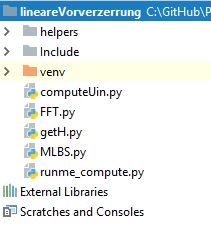
\includegraphics[scale=0.5 ]{slides/Gegeben/lineareFiles.JPG} 
	\end{textblock}	
	\begin{textblock}{20}(93,55)
    	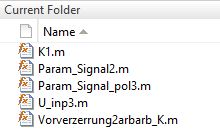
\includegraphics[scale=0.5 ]{slides/Gegeben/matlabFiles.JPG} 
	\end{textblock}	
}

}
\end{frame}


\begin{frame}
\frametitle{Code: Vorgehensweise}

\only<2->{
\begin{itemize}
	\only<1->{\item Refactoring / Anpassung der Matlab-Funktionen an unser Design}
	\only<3->{\item Portierung der Matlab-Funktionen nach Python}
	\only<4->{\item Überprüfung der portierten Funktionen mithilfe von \textbf{TDD}}
	\only<5->	
	{
		\begin{itemize}
			\item  Momentan jeweils 10 korrespondierende \textbf{Unit Tests} in Matlab und Python
		\end{itemize}
	}
	\only<6->{\item Maximale Vorbereitung der Funktionen ohne Messaufbau dank \textbf{TDD}}
	\only<7->
	{
		\begin{itemize}
			\item  Nur zum Testen von \texttt{measure\_Uout} sind Geräte notwendig
		\end{itemize}
	}		
\end{itemize}
}
 

\end{frame}


\section{Erreichtes}

\subsection{Gerätekommunikation}
\begin{frame}{Dokumentation und Gerätekommunikation  }

\begin{itemize}
	
	\item Dokumentation \uncover<2-> {: 
		\begin{itemize}
			\item Handhabung der Geräte, Vorgehensweise bei Tests
			\item Bedienung des Programms 
			\item Ausführliches Kommentieren der Code-Funktionalität
		\end{itemize}
		}
	\item Gerätekommunikation \uncover<3-> {:
		\begin{itemize}
			\item Treiber und Programmer-Manuals zur Nutzung des Programms von anderen Geräten aus 
			\item Laufzeitoptimierung durch Abfrage von Gerätezuständen mittels VISA
			\item Verbesserung der Auflösung des Signals durch Anpassung der Darstellung des Oszilloskops mittels VISA
		\end{itemize}
		}
	
	
\end{itemize}

\end{frame}





\subsection{Code}


\begin{frame}[fragile]
\ifnum\WertA=1
\frametitle{Code: Das Design}
\else
\frametitle{Code: Evaluierung}
\fi

%\only<1>
%	{ 
%\framebox{   %   % just so you can see where the "picture" is

\setcounter{onlyAt}{0}

\ifnum\WertA=1

%\setcounter{onlyAt}{\value{onlyAt}+1}
%\only<\value{onlyAt}>
%{
%	\begin{center}
%		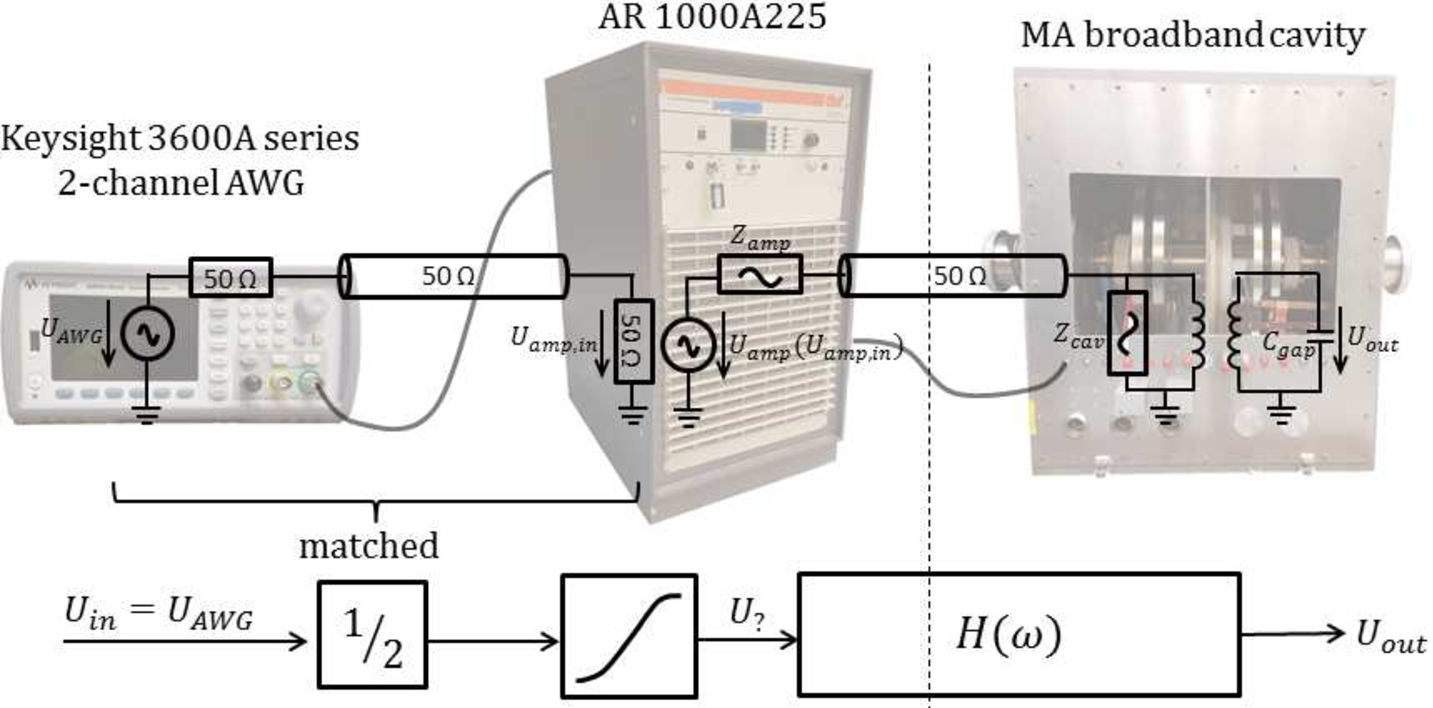
\includegraphics[scale=0.45]{slides/ResultCode/WEPVA047f2_2-eps-converted-to.pdf} 
%	\end{center}
%}

\setcounter{onlyAt}{\value{onlyAt}+1}
\only<\value{onlyAt}>
	{
	\begin{picture}(100,70)
		\put(15,0){
			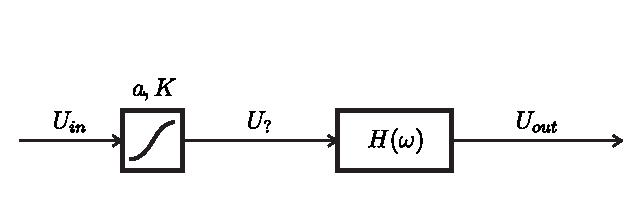
\includegraphics[scale=1.0]{slides/ResultCode/Slide1.eps} 
		}  
	\end{picture} 
	}
\fi
		
\setcounter{onlyAt}{\value{onlyAt}+1}
\only<\value{onlyAt}>
	{
	\begin{picture}(100,70)
		\put(15,0){
			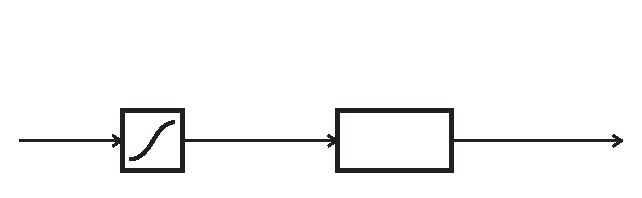
\includegraphics[scale=1.0]{slides/ResultCode/Slide2.eps} 
		}  
	\end{picture} 
	}
	


\ifnum\WertA=1 \setcounter{from}{\value{onlyAt}+1} \setcounter{till}{\value{onlyAt}+1} \else \setcounter{from}{\value{onlyAt}+1} \setcounter{till}{\value{onlyAt}+2} \fi	
\only<\value{from} - \value{till}> 
	{
	\begin{picture}(100,70)
		\put(15,0){
			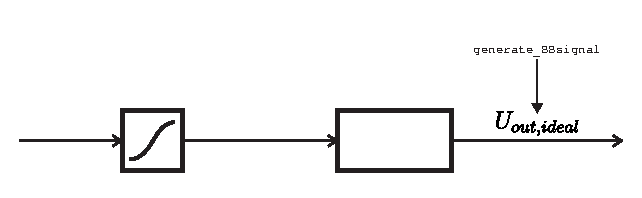
\includegraphics[scale=1.0]{slides/ResultCode/Slide3.eps} 
		}  
	\end{picture} 
	\lstinputlisting[firstline=1,lastline=1]{slides/ResultCode/file.txt} 
	}	
	
\ifnum\WertA=2
	\setcounter{onlyAt}{\value{from} + 1}
	\only<\value{onlyAt}>
	{
		\begin{textblock}{20}(80,50)
    		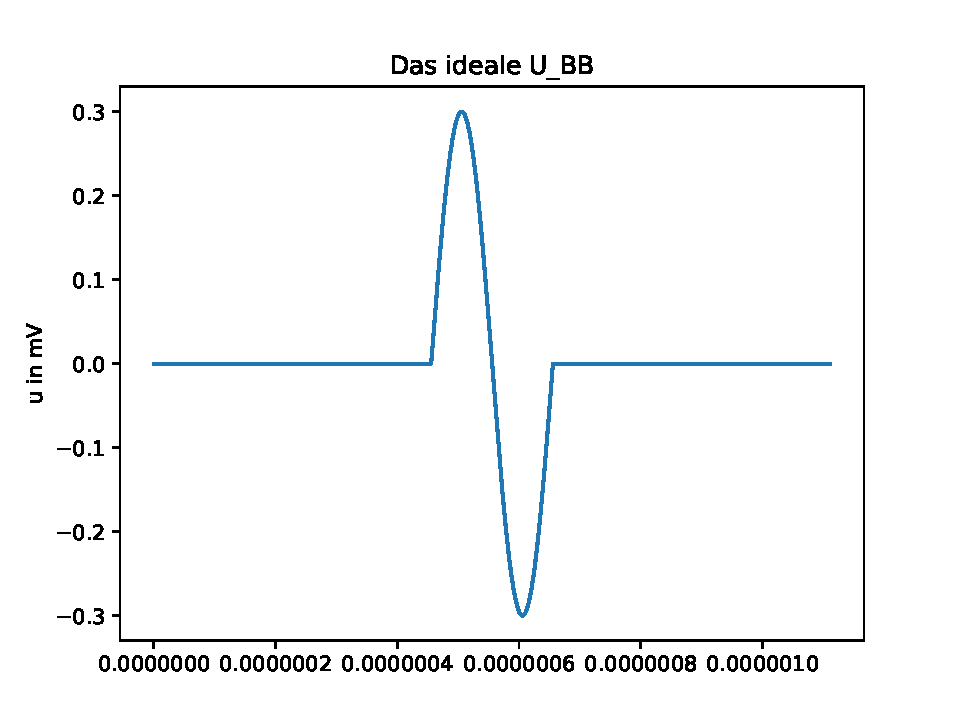
\includegraphics[height=3.5cm, width=4.5cm ]{slides/ResultCode/plots/Uout_ideal.pdf} 
		\end{textblock}	
	} 	
\fi	
\setcounter{onlyAt}{\value{till}}


\ifnum\WertA=1 \setcounter{from}{\value{onlyAt}+1} \setcounter{till}{\value{onlyAt}+1} \else \setcounter{from}{\value{onlyAt}+1} \setcounter{till}{\value{onlyAt}+2} \fi	
\only<\value{from} - \value{till}> 
	{
	\begin{picture}(100,70)
		\put(15,0){
			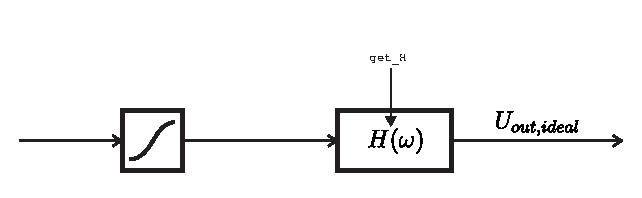
\includegraphics[scale=1.0]{slides/ResultCode/Slide4.eps} 
		}  
	\end{picture} 
	\lstinputlisting[firstline=1,lastline=2]{slides/ResultCode/file.txt} 
	}
	
\ifnum\WertA=2
	\setcounter{onlyAt}{\value{from} + 1}
	\only<\value{onlyAt}>
	{
		\begin{textblock}{20}(93,50)
    		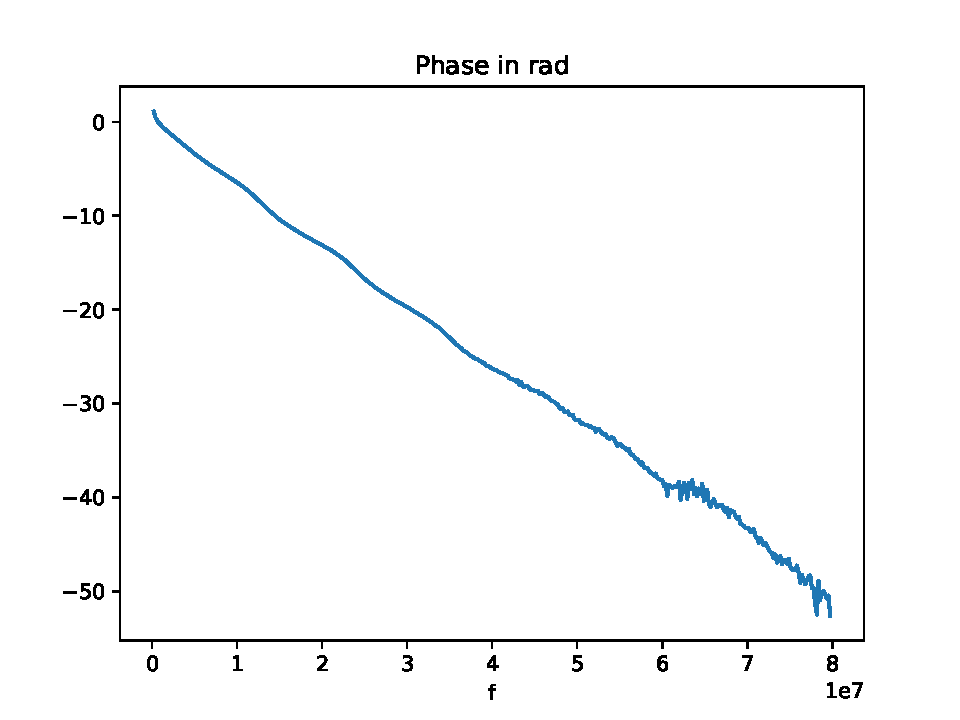
\includegraphics[ width=3.5cm, height=3.1cm ]{slides/ResultCode/plots/H_p.pdf} 
		\end{textblock}			
		\begin{textblock}{20}(61,50)
    		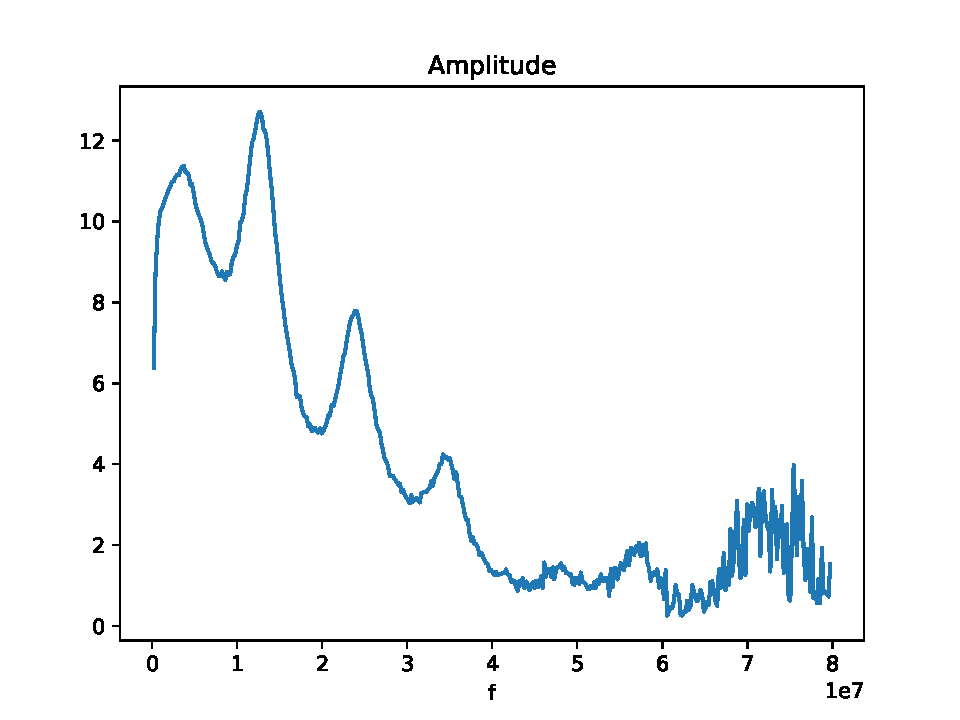
\includegraphics[ width=3.5cm, height=3.1cm]{slides/ResultCode/plots/H_a.pdf} 
		\end{textblock}	
		
	} 	 
\fi	
\setcounter{onlyAt}{\value{till}} 

\setcounter{onlyAt}{\value{onlyAt}+1}
\only<\value{onlyAt}>
	{
	\begin{picture}(100,70)
		\put(15,0){
			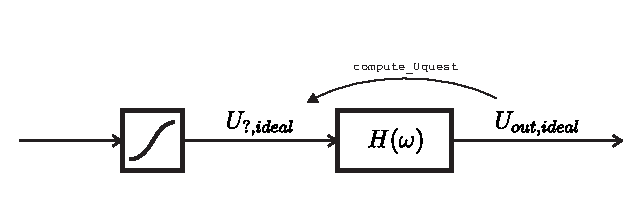
\includegraphics[scale=1.0]{slides/ResultCode/Slide5.eps} 
		}  
	\end{picture} 
	\lstinputlisting[firstline=1,lastline=3]{slides/ResultCode/file.txt} 
	}	
	
\setcounter{onlyAt}{\value{onlyAt}+1}
\only<\value{onlyAt}>
	{
	\begin{picture}(100,70)
		\put(15,0){
			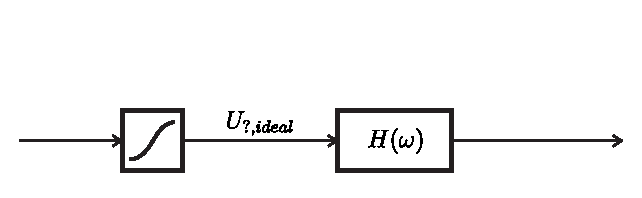
\includegraphics[scale=1.0]{slides/ResultCode/Slide5-1.eps} 
		}  
	\end{picture} 
	\lstinputlisting[firstline=1,lastline=3]{slides/ResultCode/file.txt} 
	}
	
\ifnum\WertA=2
	\setcounter{from}{\value{onlyAt}} 
	\setcounter{till}{\value{onlyAt}+2}
	\only<\value{from} - \value{till}>
	{
		\begin{textblock}{20}(80,50)
    		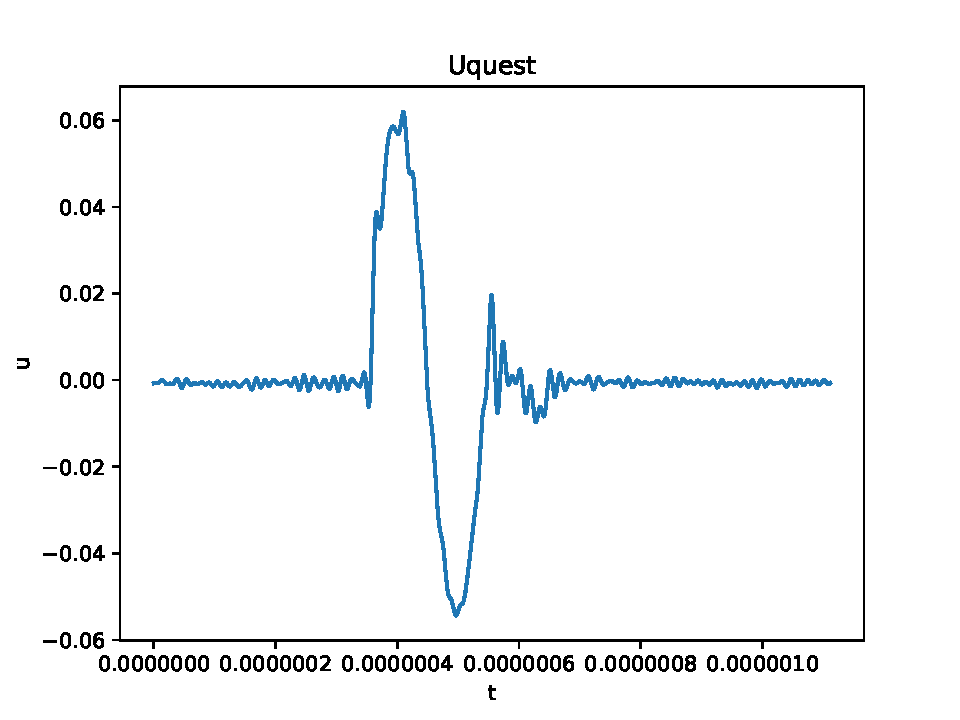
\includegraphics[height=3.5cm, width=4.5cm ]{slides/ResultCode/plots/U_quest_ideal.pdf} 
		\end{textblock}	
	} 
\fi	

\setcounter{onlyAt}{\value{onlyAt}+1}
\only<\value{onlyAt}>
{
	\begin{picture}(100,70)
		\put(15,0)
		{
			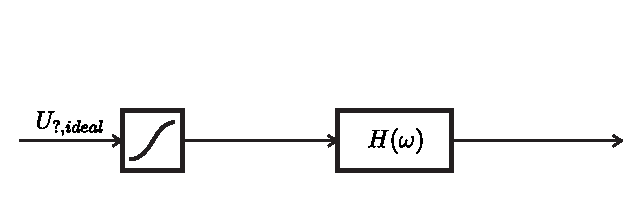
\includegraphics[scale=1.0]{slides/ResultCode/Slide6.eps} 
		}  
	\end{picture} 
	\lstinputlisting[firstline=1,lastline=3]{slides/ResultCode/file.txt} 
}

\setcounter{onlyAt}{\value{onlyAt}+1}
\only<\value{onlyAt}>
{
	\begin{picture}(100,70)
		\put(15,0)
		{
			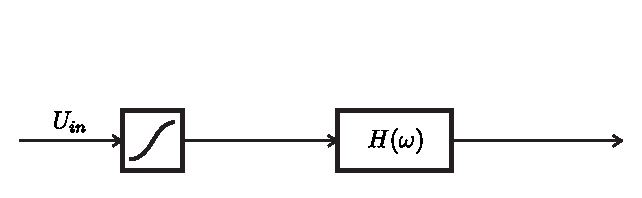
\includegraphics[scale=1.0]{slides/ResultCode/Slide7.eps} 
		}
	\end{picture} 	
	\lstinputlisting[firstline=1,lastline=4]{slides/ResultCode/file.txt} 	
}	

\setcounter{onlyAt}{\value{onlyAt}+1}
\only<\value{onlyAt}>
{
	\begin{picture}(100,70)
		\put(15,0)
		{
			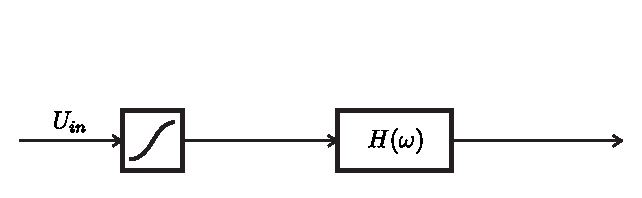
\includegraphics[scale=1.0]{slides/ResultCode/Slide7.eps} 
		}
	\end{picture} 	
	\lstinputlisting[firstline=1,lastline=5]{slides/ResultCode/file.txt} 		

}

\ifnum\WertA=1 \setcounter{from}{\value{onlyAt}+1} \setcounter{till}{\value{onlyAt}+1} \else \setcounter{from}{\value{onlyAt}+1} \setcounter{till}{\value{onlyAt}+3} \fi	
\only<\value{from} - \value{till}> 
{
	\begin{picture}(100,70)
		\put(15,0)
		{
			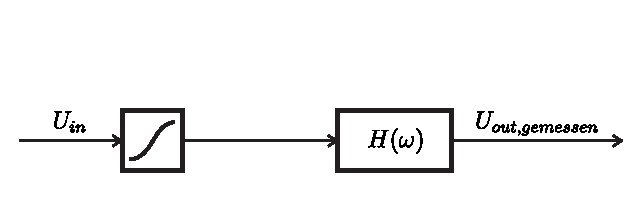
\includegraphics[scale=1.0]{slides/ResultCode/Slide8.eps} 
		}
	\end{picture} 	
	\lstinputlisting[firstline=1,lastline=5]{slides/ResultCode/file.txt} 		

}

\ifnum\WertA=2
	\setcounter{onlyAt}{\value{from}+1}
	\only<\value{onlyAt}>
	{
		\begin{textblock}{20}(80,50)
    		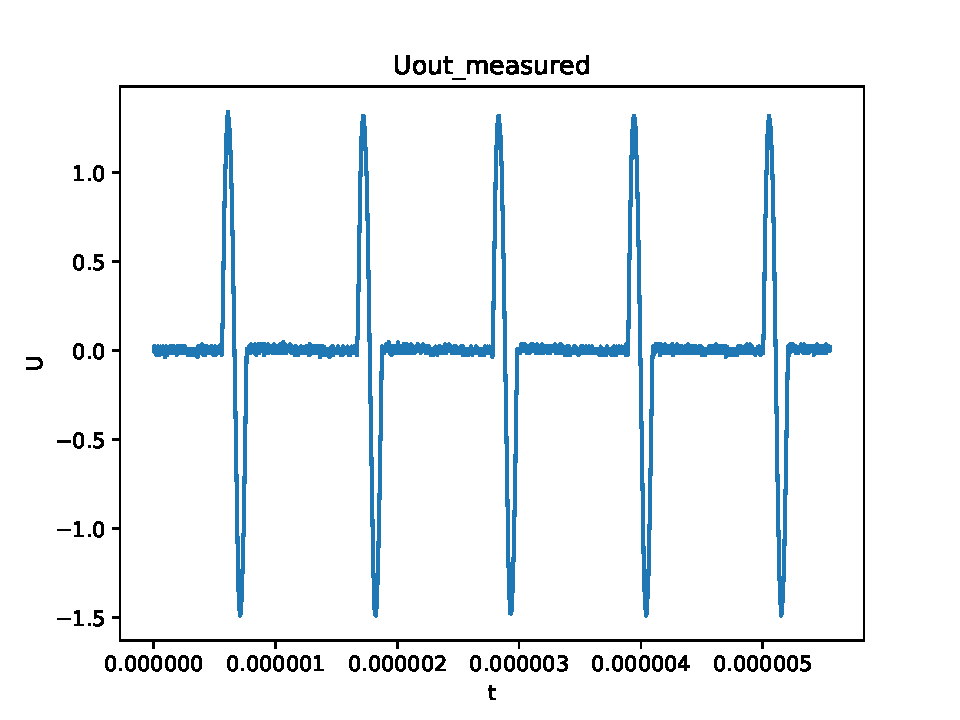
\includegraphics[height=3.5cm, width=4.5cm ]{slides/ResultCode/plots/Uout_measured.pdf} 
		\end{textblock}	
	} 
	\setcounter{onlyAt}{\value{from}+2}
	\only<\value{onlyAt}>
	{
		\begin{textblock}{20}(80,50)
    		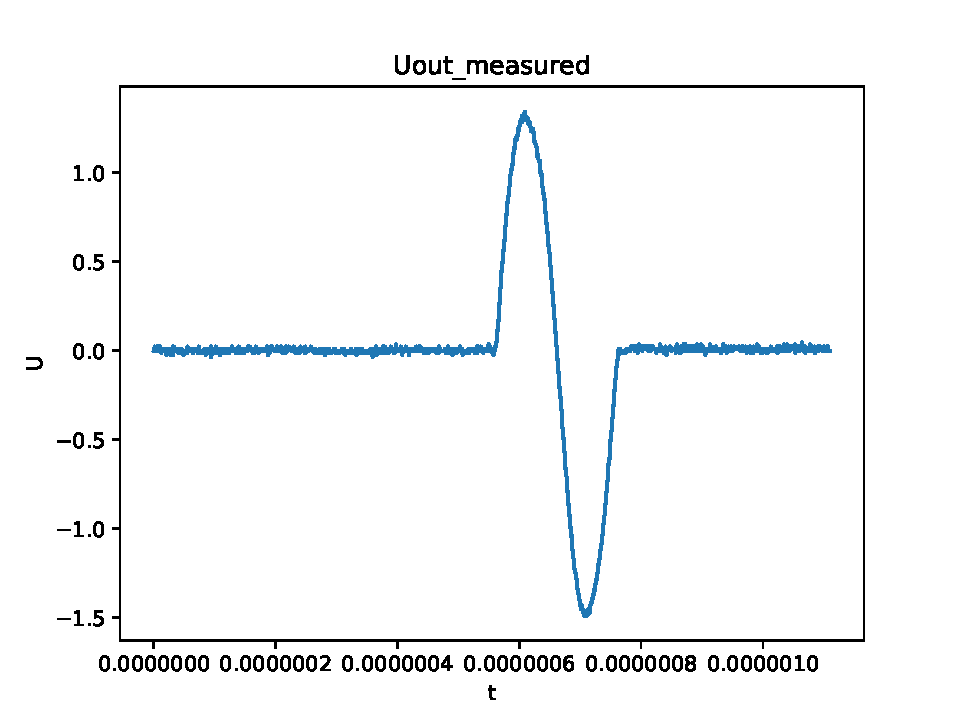
\includegraphics[height=3.5cm, width=4.5cm ]{slides/ResultCode/plots/Uout_measured_cut.pdf} 
		\end{textblock}	
	} 
\fi
\setcounter{onlyAt}{\value{till}} 
 
\ifnum\WertA=1 \setcounter{from}{\value{onlyAt}+1} \setcounter{till}{\value{onlyAt}+1} \else \setcounter{from}{\value{onlyAt}+1} \setcounter{till}{\value{onlyAt}+2} \fi	
\only<\value{from} - \value{till}> 
{
	\begin{picture}(100,70)
		\put(15,0)
		{
			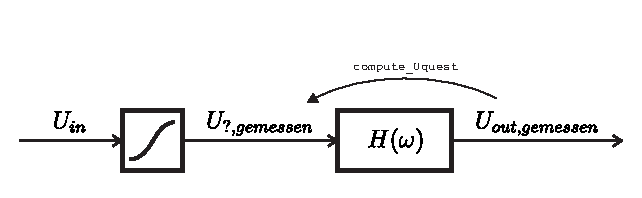
\includegraphics[scale=1.0]{slides/ResultCode/Slide9.eps} 
		}  
	\end{picture} 
	\lstinputlisting[firstline=1,lastline=6]{slides/ResultCode/file.txt} 
}	

\ifnum\WertA=2
	\setcounter{onlyAt}{\value{from} + 1}
	\only<\value{onlyAt}>
	{
		\begin{textblock}{20}(80,50)
    		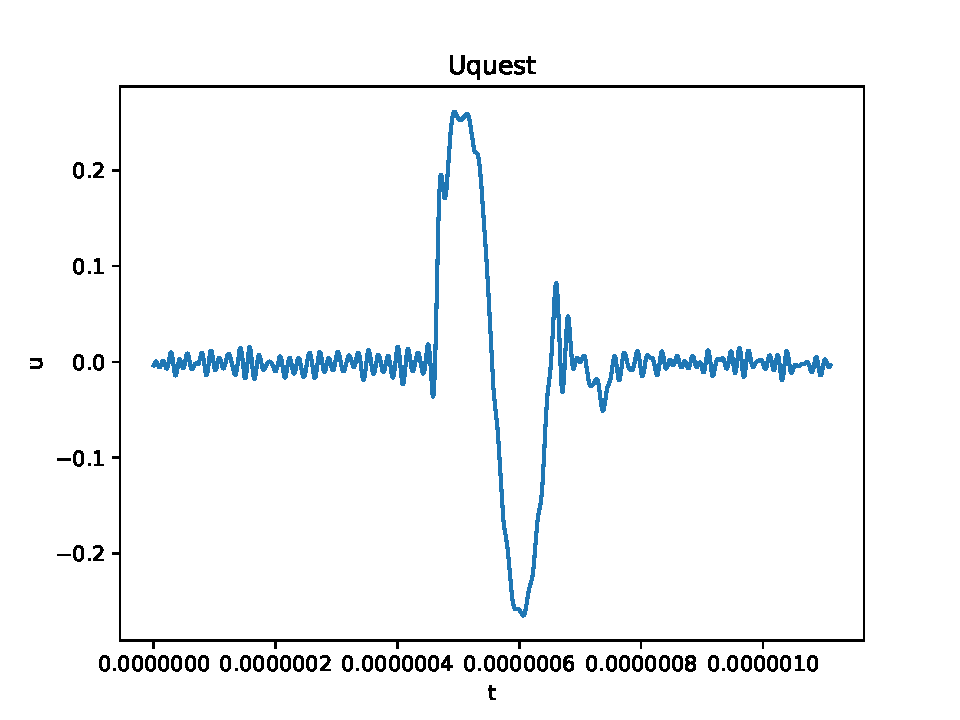
\includegraphics[height=3.5cm, width=4.5cm ]{slides/ResultCode/plots/U_quest_measured.pdf} 
		\end{textblock}	
	}
\fi
\setcounter{onlyAt}{\value{till}} 
	
\ifnum\WertA=1 \setcounter{from}{\value{onlyAt}+1} \setcounter{till}{\value{onlyAt}+1} \else \setcounter{from}{\value{onlyAt}+1} \setcounter{till}{\value{onlyAt}+2} \fi	
\only<\value{from} - \value{till}> 
{
	\begin{picture}(100,70)
		\put(15,0){
			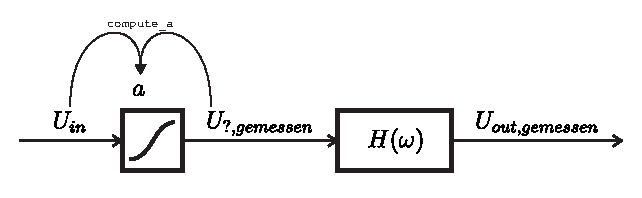
\includegraphics[scale=1.0]{slides/ResultCode/Slide10.eps} 
		}  
	\end{picture} 
	\lstinputlisting[firstline=1,lastline=7]{slides/ResultCode/file.txt} 
}

\ifnum\WertA=2
	\setcounter{onlyAt}{\value{from} + 1}
	\only<\value{onlyAt}>
	{
		\begin{textblock}{20}(65,72)
    		
\includegraphics[scale=0.6 ]{slides/ResultCode/plots/a.JPG} 
		\end{textblock}	
	} 
\fi	
\setcounter{onlyAt}{\value{till}}	


\ifnum\WertA=1 \setcounter{from}{\value{onlyAt}+1} \setcounter{till}{\value{onlyAt}+1} \else \setcounter{from}{\value{onlyAt}+1} \setcounter{till}{\value{onlyAt}+2} \fi	
\only<\value{from} - \value{till}> 
{
	\begin{picture}(100,70)
		\put(15,0)
		{
			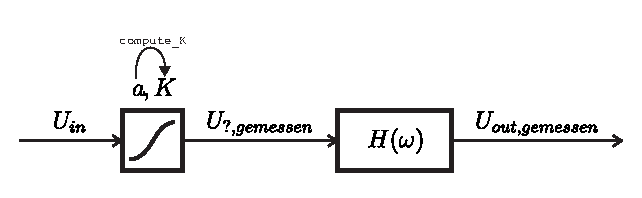
\includegraphics[scale=1.0]{slides/ResultCode/Slide11.eps} 
		}  
	\end{picture} 
	\lstinputlisting[firstline=1,lastline=8]{slides/ResultCode/file.txt} 
}

\ifnum\WertA=2
	\setcounter{onlyAt}{\value{from} + 1}
	\only<\value{onlyAt}>
	{
		\begin{textblock}{20}(80,50)
    		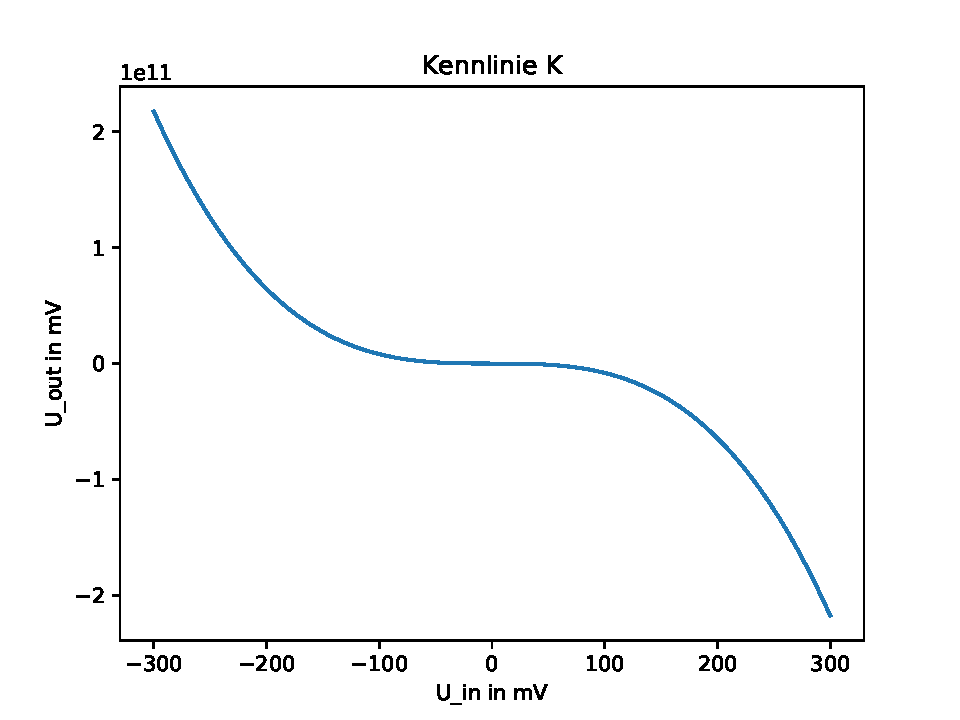
\includegraphics[height=3.5cm, width=4.5cm ]{slides/ResultCode/plots/K.pdf} 
		\end{textblock}	
	} 
\fi	
\setcounter{onlyAt}{\value{till}}	

\setcounter{onlyAt}{\value{onlyAt}+1}
\only<\value{onlyAt}>
{
	\begin{picture}(100,70)
		\put(15,0)
		{
			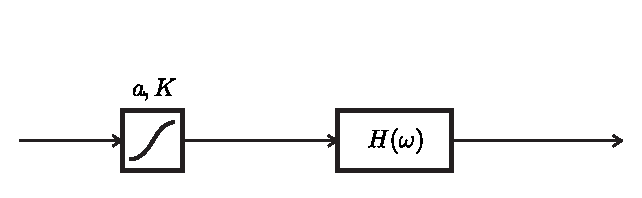
\includegraphics[scale=1.0]{slides/ResultCode/Slide12-0.eps} 
		}  
	\end{picture} 
	\lstinputlisting[firstline=1,lastline=8]{slides/ResultCode/file.txt} 
}
	
\setcounter{onlyAt}{\value{onlyAt}+1}
\only<\value{onlyAt}>
{
	\begin{picture}(100,70)
		\put(15,0)
		{
			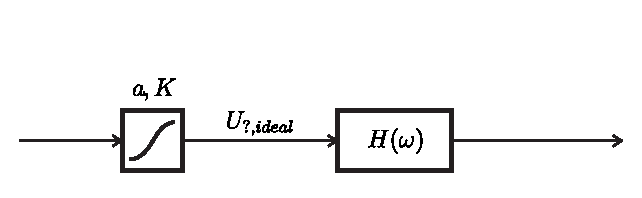
\includegraphics[scale=1.0]{slides/ResultCode/Slide12-01.eps} 
		}  
	\end{picture} 
	\lstinputlisting[firstline=1,lastline=8]{slides/ResultCode/file.txt} 
}
	
\ifnum\WertA=1 \setcounter{from}{\value{onlyAt}+1} \setcounter{till}{\value{onlyAt}+1} \else \setcounter{from}{\value{onlyAt}+1} \setcounter{till}{\value{onlyAt}+2} \fi	
\only<\value{from} - \value{till}> 
{
	\begin{picture}(100,70)
		\put(15,0)
		{
			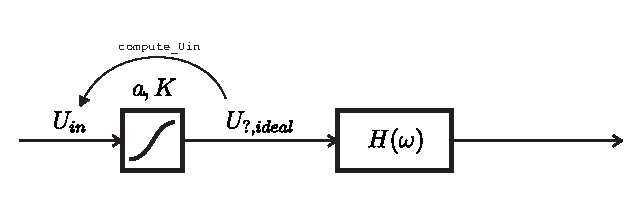
\includegraphics[scale=1.0]{slides/ResultCode/Slide12.eps} 
		}  
	\end{picture} 
	\lstinputlisting[firstline=1,lastline=9]{slides/ResultCode/file.txt} 
}

\ifnum\WertA=2
	\setcounter{onlyAt}{\value{from} + 1}
	\only<\value{onlyAt}>
	{
		\begin{textblock}{20}(80,50)
    		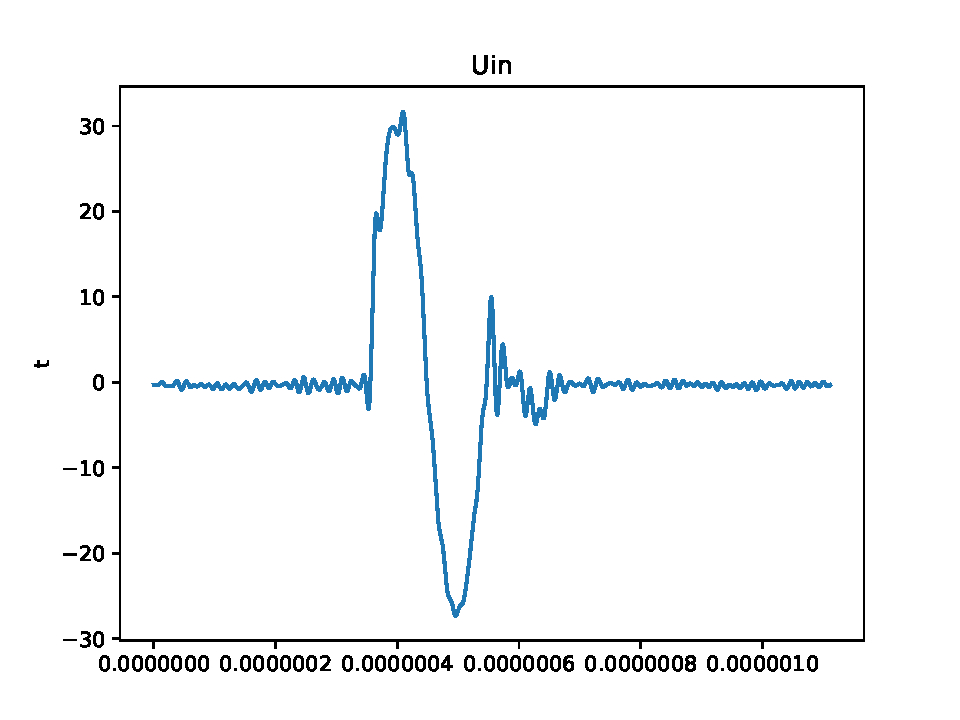
\includegraphics[height=3.5cm, width=4.5cm ]{slides/ResultCode/plots/U_in.pdf} 
		\end{textblock}	
	} 
\fi	
\setcounter{onlyAt}{\value{till}}
	
\setcounter{onlyAt}{\value{onlyAt}+1}
\only<\value{onlyAt}>
{
	\begin{picture}(100,70)
		\put(15,0)
		{
			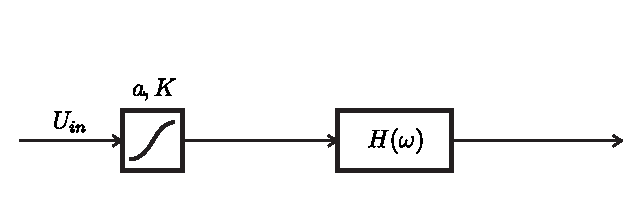
\includegraphics[scale=1.0]{slides/ResultCode/Slide13-0.eps} 
		}  
	\end{picture} 
	\lstinputlisting[firstline=1,lastline=9]{slides/ResultCode/file.txt} 
}



%\setcounter{onlyAt}{\value{onlyAt}+1}
%\only<\value{onlyAt}>
%{
%	\begin{picture}(100,70)
%		\put(15,0)
%		{
%			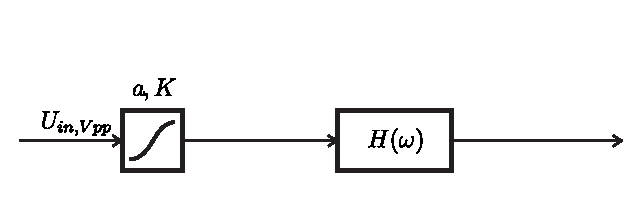
\includegraphics[scale=1.0]{slides/ResultCode/Slide13-01.eps} 
%		}  
%	\end{picture} 
%	\lstinputlisting[firstline=1,lastline=10]{slides/ResultCode/file.txt} 
%}
	
\setcounter{onlyAt}{\value{onlyAt}+1}
\only<\value{onlyAt}>
{
	\begin{picture}(100,70)
		\put(15,0)
		{
			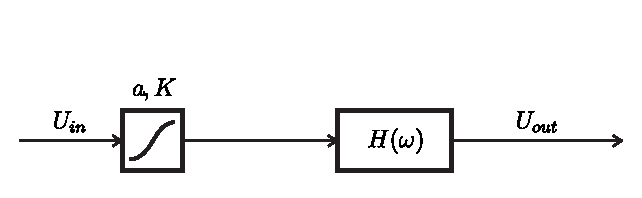
\includegraphics[scale=1.0]{slides/ResultCode/Slide13.eps} 
		}  
	\end{picture} 
	\lstinputlisting[firstline=1,lastline=10]{slides/ResultCode/file.txt} 
}

  
%	\begin{figure}[t]
%	
%%	
%	\end{figure}	
	%}
%\only<2>{ \lstinputlisting[firstline=1,lastline=2]{slides/ResultCode/file.txt} }
%\only<3>{ \lstinputlisting[firstline=1,lastline=3]{slides/ResultCode/file.txt} }
%\only<4>{ \lstinputlisting[firstline=1,lastline=4]{slides/ResultCode/file.txt} }
%\only<5>{ \lstinputlisting[firstline=1,lastline=5]{slides/ResultCode/file.txt} }
%\only<6>{ \lstinputlisting[firstline=1,lastline=6]{slides/ResultCode/file.txt} }
%\only<7>{ \lstinputlisting[firstline=1,lastline=7]{slides/ResultCode/file.txt} }
%\only<8>{ \lstinputlisting[firstline=1,lastline=8]{slides/ResultCode/file.txt} }
%\only<9>{ \lstinputlisting[firstline=1,lastline=9]{slides/ResultCode/file.txt} }
%\only<10>{ \lstinputlisting[firstline=1,lastline=10]{slides/ResultCode/file.txt} }


\end{frame}





\section{Evaluierung}
\subsection{Gerätekommunikation}
\begin{frame}{Evaluierung: Dokumentation und Gerätekommunikation}

%Stand letzter Test
Unvollständige Dokumentation:
\begin{itemize}
	\item Ausführliche Beschreibung von In- und Output-Formaten von Methoden
	\item Begründung von nicht-trivialen Umformungsschritten in Methoden
\end{itemize}

Getestet und funktionsfähige Aspekte der Gerätekommunikation:
\begin{itemize}
	\item VISA-Protokoll und PyVisa Package Installation 
	\item Kommunikation mit AWG von anderem Laptop aus über USB
\end{itemize}

Noch nicht erfolgreich getestete Aspekte der Gerätekommunikation:
\begin{itemize}
	\item Kommunikation mit Oszilloskop von anderem Laptop aus über LAN
	\item Laufzeit: Status-Abfrage der Geräte mit \lstinline{BUSY?} oder \lstinline{*WAI}
	\item Anpassung der Auflösung [\textit{noch nicht implementiert}]
\end{itemize}

\end{frame}





\subsection{Code}
\begin{frame}{Evaluierung: Python-Code für die nichtlinere Verzerrung}

\end{frame}





\section{Ausblick}
\documentclass[../Report.tex]{subfiles}


\begin{document}


\chapter{Ausblick}
\label{chap:ausb}
---- In diesem Kapitel wird auf offene Fragen / neue Probleme / Anstöße für weitere Arbeiten eingegangen. Dabei sollte es um eher inhaltliche Aspekte gehen (u. U. wenig to dos für Code-Design) gegebenenfalls darf hier bei vielem auf die Erfahrungen aus den vorigen Kapiteln verwiesen werden und damit einen Übersichts-Charakter haben (erleichtert nachfolgenden Projekten die Arbeit) --- 

\section{Impressionen zum Code}
\label{sec:ausb.code}
In Bezug auf das Design des Codes verbleiben eine Reihe Anregungen und Gedanken, die nicht realisiert wurden, je nach Ausführung aber interessant zu bedenken sein könnten.

\begin{itemize}
	\item	Die Geräte AWG und DSO als Klassen einzubinden könnte den Vorteil bieten, alle SCPI Commands an einer Stelle zu bündeln und den Zugriff darauf allgemeingültig zu halten.
	
	\item	Eine Einbindung des momentanen Programms in die RF-Tools des GSI-Standards könnte in zwei Teilen erfolgen. Die bestehende Funktionalität zur Berechnung von $K$ und $\Hcompl$ kann unabhängig der Optimierungsalgorithmen genutzt werden. Dabei ist insbesondere zu prüfen, ob oder wie die Aspekte im \nameref{chap:code} beibehalten werden. 
	
	\item 	Die momentane Version ist in erster Linie über eine Python-IDE ausführbar. Die Ausführung über die Kommandozeile wurde nicht fokussiert.
	\item Für die Erstellung eines idealen Barrier-Bucket Ausgangssignals wird momentan noch eine selbst implementierte Methode verwendet. Dafür kann auch das vorhandene RF-Tool verwendet werden.
	
\end{itemize}





\section{Ausblick: Optimierung}
\label{sec:ausb.opti}

- (offene Punkte K-Optimierung?)


Auf den Ergebnissen aus \nameref{chap:opt} aufbauend, verbleiben eine Reihe von offenen Fragestellungen:

\begin{enumerate}
	\item 	Wie wirkt sich die Optimierung von $K$ aufgrund ihrer Nichtlinearität auf die Übertragungsfunktion $\Hcompl$ aus und muss dies in der Optimierung berücksichtigt werden, etwa in der Reihenfolge der Iterationsschritte?
	
	\item	Wie wird mit der Tatsache umgegangen, dass im Frequenzbereich unabhängig der Qualität der Messung nur etwa halb so viele Daten für die Anpassung zur Verfügung stehen, wie in $\Hcompl$ selbst vorliegen?
	
	\item 	Ist die getrennte Interpolation von Betrag und Phase der Signalspektren auf die Frequenzen der Übertragungsfunktion in der Optimierung von $\Hcompl$ die beste Lösung? 
	
	\item	In welcher Reihenfolge wird die Iteration durchgeführt? Wird zuerst $\Hcompl$ in mehreren Durchgängen angepasst und danach $K$? Oder im Wechsel je eine Iteration?
	
	\item 	Wie wird die Auswahl der Schrittweiten $\sigma_H$ und $\sigma_a$ vorgenommen? Werden diese pauschal einmal festgesetzt zu Beginn des Algorithmus oder ist eine dynamische Anpassung, etwa durch die Qualität des letzten gemessenen Signals oder in Abhängigkeit des Iterationsschritts vorzuziehen? 
	
	\item 	Wie lässt sich der Einfluss von zufälligem Rauschen auf die Optimierung reduzieren? Insbesondere die Auflösung im höherfrequenten Betragsspektrum ist hier problematisch. Und im Falle des Ignorieren von Korrekturen an als fehlerhaft befundenen Frequenzen: Auf welchen Wert wird der Korrekturterm bei diesen Frequenzen gesetzt?
	
	\item	Wie lassen sich die im idealen Spektrum des Einzelsinus enthaltenen Nulldurchgänge in der Optimierung von $\Hcompl$ berücksichtigen, um interpolationsbedingt große Fehlerterme zu vermeiden? Ist das einfache Ignorieren dieser Frequenzen für die Anpassung eine Möglichkeit? Und in welchem kleinen Frequenzbereich um einen Nulldurchgang müssten dann die Werte ignoriert werden?
	
	\item 	Wie - insofern überhaupt - ist eine Optimierung der Phase von $\Hcompl$ zu gestalten?
	
	\item	Nach welchem Qualitätsmerkmal wird das Signal bewertet und wie wirkt sich dies auf den Algorithmus aus?
	
	\item	Gibt es eine sinnvolle Abbruchbedingung, mit der die Iteration versehen werden sollte? Etwa, dass sich die Qualität im Vergleich zu den vorherigen Iterationen nicht mehr mit ähnlicher Rate verbessert hat? Der Trade-Off liegt zwischen Laufzeit und Signal-Qualität.
	
	\item	Wie bestimmt man die Grenzen, in denen $K$ genutzt werden kann? Wie kann man garantieren, dass $K$ in den Bereichen, aus denen die Daten zur Berechnung von $a_n$ benutzten werden, bijektiv ist?
	
	\item	Gibt es eine Möglichkeit die Grenzen von $K$ bei der Optimierung zu erweitern? Ein möglicher Indikator: Kann man die Rückgabe von \lstinline{numpy.linalg.lstsq(LGS)} aus der Berechnung von $a_n$ nutzen, um eine Aussage über die Abweichung der Werte zu treffen?
\end{enumerate}





\section{--- Gerätekomm---}
\label{sec:ausb.geraete}
--- in dieser Section werden weitere Punkte der Geräte-Komm aufgegriffen, etwa - die (geringe) Auflösung des AWG im Kontext der Optimierung (ggf. in \ref{sec:ausb.opti} besser?) , die Einbindung des neuen Oszis oder die Idee der Klassen-Implementierung 
%TODO: prüfe Redundanz mit Abschnitt Gerätekommunikation! nur eine Einbindung, wo ist sie sinnvoller? 

%TODO: Überlegung ausführen, ob RF-Tools einbinden hier sinnvoller ist als in "Offenen Fragen" im Abschnitt Code-Design?






\end{document}
	
	
\end{document}